% Number 680
% CopM pTM ETM Algebra Units Vectors
% Superman stopping train
% MIT/JG

% Watermark
\AddToShipoutPicture*{\BackgroundPic}

\addtocounter {ProbNum} {1}

%\begin{floatingfigure}[r]{.4\textwidth}
%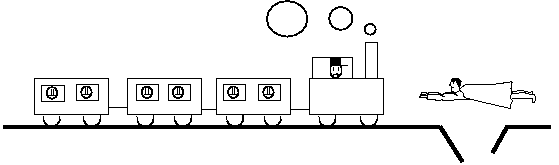
\includegraphics[scale=.6]{/Users/jgates/desktop/latex/pics/superman1}
%\end{floatingfigure}
 
{\bf \Large{\arabic{ProbNum}}} Find the speed at which Superman 86 kg must fly into a train 19,600 kg traveling at ${80~\tfrac{km}{hr}}$ in order to stop it.

\hspace{30 mm} 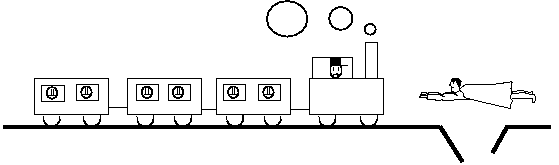
\includegraphics[scale=.5]{/Users/jgates/desktop/latex/pics/superman1} 

\vfill
Running into the train at that speed would severely damage both train and passengers. Calculate the minimum time Superman must take to stop the train, if the passengers experience an average horizontal force of $43\%$ of their own weight.

\vfill	
How far does the train then travel while being slowed to a stop?

\vfill
%\hfill 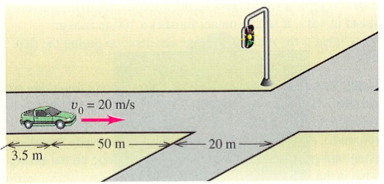
\includegraphics[scale=.85]{/Users/jgates/desktop/latex/pics/redlight.png}
\newpage